\documentclass[../../main/main.tex]{subfiles}
\graphicspath{{./figures/}}

\makeatletter
\renewcommand{\@chapapp}{Optique -- chapitre}
\makeatother

% \toggletrue{student}
% \HideSolutionstrue

\begin{document}
\setcounter{chapter}{1}

\chapter{\switch{TD~: Base de l'optique g\'eom\'etrique}{Correction du TD}}

\section{Fréquence, longueur d'onde et indice}
\switch{
	La lumière visible possède des longueurs d'onde dans le vide comprises entre
	\SIrange{400}{800}{nm}.
	\begin{enumerate}
		\item À quel intervalle de fréquences cela correspond-il~?
		\item Que deviennent ces longueurs d'ondes
		      \begin{enumerate}
			      \item dans l'eau d'indice $n_1 = \num{1.33}$~?
			      \item dans un verre d'indice $n_2 = \num{1.5}$~?
		      \end{enumerate}
		\item Calculer la valeur de la vitesse de la lumière dans un verre d'indice
		      $n = \num{1.5}$.
	\end{enumerate}
}{
	\begin{enumerate}
		\item On définit $\lambda_{r,0} = \SI{800}{nm}$ et $\lambda_{b,0} =
			      \SI{400}{nm}$ les longueurs d'ondes dans le vide correspondant au
		      extrémités bleue et rouge du spectre de la lumière visible.\bigbreak
		      On sait que
		      \begin{equation*}
			      f = \frac{c}{\lambda_0}
		      \end{equation*}
		      On aura donc\smallbreak
		      \begin{minipage}{0.45\linewidth}
			      \begin{empheq}[box=\fbox]{align*}
				      f_b &= \frac{c}{\lambda_{b,0}}\\
				      f_r &= \frac{c}{\lambda_{r,0}}
			      \end{empheq}
		      \end{minipage}
		      \begin{minipage}{0.45\linewidth}
			      \begin{equation*}
				      \text{avec}\quad
				      \left\{
				      \begin{array}{rcl}
					      c             & = & \SI{3.00e8}{m.s^{-1}}          \\
					      \lambda_{b,0} & = & \SI{400}{nm} = \SI{4.00e-7}{m} \\
					      \lambda_{r,0} & = & \SI{800}{nm} = \SI{8.00e-7}{m}
				      \end{array}
				      \right.
			      \end{equation*}
		      \end{minipage}\smallbreak
		      L'application numérique donne
		      \begin{empheq}[box=\fbox]{align*}
			      f_b &= \SI{7.50e14}{Hz} = \SI{750}{THz}\\
			      f_r &= \SI{3.80e14}{Hz} = \SI{380}{THz}
		      \end{empheq}
		\item Dans un milieu TLHI, la longueur d'onde change de valeur selon
		      \begin{equation*}
			      \lambda = \frac{\lambda_0}{n}
		      \end{equation*}
		      Ainsi,
		      \begin{enumerate}
			      \item dans l'eau d'indice $n_1 = \num{1.33}$,
			            \begin{empheq}[box=\fbox]{align*}
				            \lambda_{b,\rm eau} &= \SI{300}{nm} \\
				            \lambda_{r,\rm eau} &= \SI{602}{nm}
			            \end{empheq}
			      \item dans un verre d'indice $n_2 = \num{1.5}$,
			            \begin{empheq}[box=\fbox]{align*}
				            \lambda_{b,\rm eau} &= \SI{267}{nm} \\
				            \lambda_{r,\rm eau} &= \SI{533}{nm}
			            \end{empheq}
		      \end{enumerate}
		      Leur couleur ne change cependant pas puisque \textbf{la couleur d'une
			      lumière est définie par sa fréquence/longueur d'onde dans le vide}.
		\item Dans un milieu TLHI, la vitesse de la lumière se calcule avec
		      \begin{equation*}
			      v = \frac{c}{n}
		      \end{equation*}
		      Avec $n = \num{1.5}$, on a donc
		      \begin{empheq}[box=\fbox]{equation*}
			      v = \SI{2.00e8}{m.s^{-1}}
		      \end{empheq}
	\end{enumerate}
}

\section{Détermination directe de l'indice d'un liquide}
\switch{
	\noindent
	\begin{minipage}[c]{.68\linewidth}
		Un rayon lumineux dans l'air ($n_{\rm air}$) tombe sur la surface horizontale
		d'un liquide d'indice $n$. Il fait un angle $\alpha = \ang{56;;}$ avec le plan
		horizontal. La déviation entre le rayon incident et le rayon réfracté est
		$\theta = \ang{13.5;;}$. Quel est l'indice $n$ du liquide~?
	\end{minipage}
	\hfill
	\begin{minipage}[c]{.3\linewidth}
		~
		% \vspace{-20pt}
		\begin{center}
			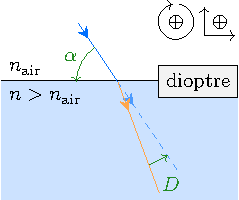
\includegraphics[width=\linewidth]{dioptre_alpha-horiz_plain}
			\label{fig:alpha_horiz}
		\end{center}
	\end{minipage}
}{
	Cet exercice est d'une simplicité absolue. Et pourtant...
	\begin{tcb}[sidebyside, righthand ratio=.45](data){Données}
		\begin{enumerate}
			\item Rayon incident sur un dioptre entre air et milieu d'indice $n$ :
			      angle {\huge avec le dioptre} de \ang{56;;} ;
			\item Différence d'angle entre rayon incident et réfléchi (« déviation
			      ») de \ang{13.5;;}.
		\end{enumerate}
		\tcblower
		\begin{center}
			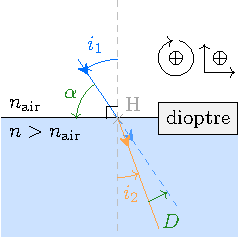
\includegraphics[width=5cm]{dioptre_alpha-horiz.pdf}
		\end{center}
	\end{tcb}
	\begin{tcbraster}[raster columns=6, raster equal height=rows]
		\begin{tcb}[raster multicolumn=2](ques){Résultat attendu}
			Indice du liquide.
		\end{tcb}
		\begin{tcb}[raster multicolumn=4](tool)'r'{Outils du cours}
			Loi de \textsc{Snell-Descartes}~:
			\[
				\boxed{n_1\sin i_1 = n_2 \sin i_2}
			\]
			avec $n_1$ l'indice du milieu d'incidence, $n_2$ celui du milieu
			de réfraction, $i_1$ l'angle d'incidence et $i_2$ l'angle de
			réfraction.
		\end{tcb}
	\end{tcbraster}

	\begin{tcb}(appl){Application}
		Un bon schéma fait attentivement est \textbf{nécessaire} ici. En effet,
		les angles donnés ne sont pas ceux qu'on utilise dans la relation de
		\textsc{Snell-Descartes}. \bigbreak

		En appelant $\alpha$ l'angle entre le rayon et le dioptre, on a
		\[ \alpha + i_1 = \ang{90;;}\]
		donc \fbox{$i_1 = \ang{34;;}$}. Et en appelant $D$ la déviation entre
		les deux rayons, on a
		\[ i_1 = i_2 + D\]
		soit \fbox{$i_2 = \ang{20.5;;}$}. On en déduit donc
		\[\boxed{n = \frac{\sin i_1}{\sin i_2}} \quad \text{avec} \quad
			\left\{
			\begin{array}{rcl}
				i_1 & = & \ang{34;;}   \\
				i_2 & = & \ang{20.5;;}
			\end{array}
			\right. \quad \text{soit} \quad \boxed{n = 1.6}
		\]
	\end{tcb}
}

\section{Détecteur de pluie sur un pare-brise}
\switch{
	\begin{wrapfigure}[8]{R}{.3\linewidth}
		\vspace*{10pt}
		\centering
		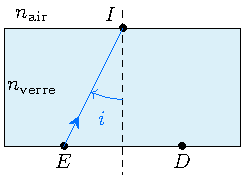
\includegraphics[width=\linewidth]{pluie_plain.pdf}
		\label{fig:pluie_plain}
	\end{wrapfigure}
	On modélise un pare-brise par une lame de verre à faces parallèles, d'épaisseur
	$e = \SI{5.00}{mm}$, d'indice $n_v = \num{1.5}$. Un fin pinceau lumineux issu d'un
	émetteur situé en E arrive de l'intérieur du verre sur le dioptre verre
	$\rightarrow$ air en I avec un angle d'incidence $i = \ang{60.;;}$.
	\begin{enumerate}
		\item Montrer que le flux lumineux revient intégralement sur le détecteur
		      situé en D et déterminer la distance ED.
		\item Lorsqu'il pleut, une lame d'eau d'indice $n_e = \num{1.33}$ et
		      d'épaisseur $e' = \SI{1.00}{mm}$ se dépose sur un pare-brise. Représenter
		      le rayon lumineux dans ce cas. À quelle distance du détecteur
		      arrive-t-il~?
	\end{enumerate}
}{
	On modélise un pare-brise par une lame de verre à faces parallèles, d'épaisseur
	$e = \SI{5.00}{mm}$, d'indice $n_v = \num{1.5}$. Un fin pinceau lumineux issu d'un
	émetteur situé en E arrive de l'intérieur du verre sur le dioptre verre
	$\rightarrow$ air en I avec un angle d'incidence $i = \ang{60.;;}$.
	\begin{enumerate}
		\item Pour savoir si le pinceau lumineux revient intégralement, il faut
		      savoir s'il y a réflexion totale à l'interface verre$\rightarrow$air.
		      Pour cela, on utilise la formule de l'angle limite de réfraction
		      \begin{equation*}
			      i_{\rm lim} = \arcsin \left( \frac{n_2}{n_1} \right)
		      \end{equation*}
		      Ici, on a
		      \[\boxed{i_{\rm lim, v\rightarrow a} =
				      \arcsin \left( \frac{n_{\rm air}}{n_{\rm verre}} \right)}
			      \quad\text{avec}\quad
			      \left\{
			      \begin{array}{rcl}
				      n_{\rm air}   & = & \num{1.00} \\
				      n_{\rm verre} & = & \num{1.5}
			      \end{array}
			      \right.
		      \]
		      L'application numérique donne
		      \begin{empheq}[box=\fbox]{equation*}
			      i_{\rm lim, v\rightarrow a} = \ang{41.8;;}
		      \end{empheq}
		      Comme $i = \ang{60.;;}$, $i > i_{\rm lim v\rightarrow a}$, et on a
		      donc réflexion totale~: aucun rayon ne sera réfracté.\bigbreak
		      Avec la figure ci-après, on a $\tan(i) = \frac{\\rm  ED}{2e}$, soit
		      \[\boxed{{\rm ED} = 2e\tan(i)}
			      \quad\text{avec}\quad
			      \left\{
			      \begin{array}{rcl}
				      e & = & \SI{5.00}{mm} \\
				      i & = & \ang{60.;;}
			      \end{array}
			      \right.\]
		      L'application numérique donne
		      \begin{empheq}[box=\fbox]{equation*}
			      ED = \SI{1.7}{cm}
		      \end{empheq}
		\item Dans le cas où une fine couche d'eau recouvre le verre, on doit
		      calculer le nouvel angle limite de réfraction pour l'interface
		      verre$\rightarrow$eau. Comme précédemment, on utilise la formule et on
		      trouve
		      \begin{empheq}[box=\fbox]{equation}
			      i_{\rm lim, v\rightarrow e} = \ang{62.5;;}
		      \end{empheq}
		      Cette fois, l'angle d'incidence $i < i_{\rm lim, v\rightarrow e}$. On
		      va donc avoir réfraction. On détermine l'angle de réfraction $i_2$
		      avec la loi de \textsc{Snell-Descartes} pour la réfraction~:
		      $n_2\sin(i_2) = n_1\sin(i_1)$. Dans notre cas, $n_2 = n_{\rm eau}$,
		      $n_1 = n_{\rm verre}$ et $i_1 = i$~; on aura donc
		      \[
			      \boxed{i_2 = \arcsin \left(
				      \frac{n_{\rm verre}\sin(i)}{n_{\rm eau}}
				      \right)}
			      \quad\text{avec}\quad
			      \left\{
			      \begin{array}{rcl}
				      n_{\rm verre} & = & \num{1.5}   \\
				      i             & = & \ang{60.;;} \\
				      n_{\rm eau}   & = & \num{1.33}
			      \end{array}
			      \right.
		      \]
		      D'où
		      \begin{empheq}[box=\fbox]{equation*}
			      i_2 = \ang{77.6;;}
		      \end{empheq}
		      Ce rayon réfracté (en vert sur la figure) va ensuite rencontrer le
		      dioptre eau$\rightarrow$air en $J$, pour lequel l'angle limite de
		      réfraction est
		      \begin{empheq}[box=\fbox]{equation*}
			      i_{\rm lim, e\rightarrow a} = \ang{48.8;;}
		      \end{empheq}
		      Comme $i_2 > i_{\rm lim, e\rightarrow a}$, on a une nouvelle réflexion
		      totale avec $r=-i_2$, ramenant le pinceau vers le dioptre
		      eau$\rightarrow$verre en un point K. Dans cette situation comme la
		      valeur absolue de $r$ est la même que celle de $i_2$, le principe
		      du retour inverse de la lumière nous permet de déterminer directement
		      que l'angle de réfraction de l'eau vers le verre $i_3$ a la même valeur
		      absolue que l'angle d'incidence du verre vers l'eau $i_1$.\bigbreak

		      Avec le schéma ci-après, on peut déterminer que $\rm DL = IK$
		      (l'abscisse supplémentaire du trajet dans l'eau) et utiliser la
		      trigonométrie pour trouver
		      \[
			      \boxed{{\rm IK} = 2e'\tan(i_2)}
			      \quad\text{avec}\quad
			      \left\{
			      \begin{array}{rcl}
				      e'  & = & \SI{1.00}{mm} \\
				      i_2 & = & \ang{77.6;;}
			      \end{array}
			      \right.\]
		      soit
		      \[
			      \boxed{{\rm DL} = \SI{0.9}{cm}}
		      \]
		      Ainsi, le rayon ne tombe plus sur le détecteur mais à côté~; un système
		      de commande relié au détecteur peut alors déclencher les essuie-glaces.
	\end{enumerate}
	\begin{figure}[h]
		\centering
		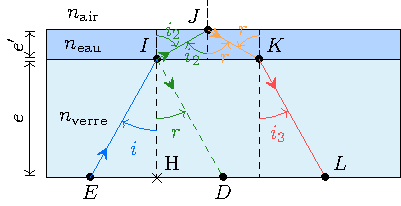
\includegraphics[width=\linewidth]{pluie.pdf}
		\label{fig:pluie_plain}
	\end{figure}
}

\section{Rayon lumineux à travers une vitre}
\switch{
	Un rayon lumineux traverse une vitre d'épaisseur $a = \SI{5.0}{mm}$ et d'indice
	$n = \num{1.5}$ sous une incidence $i_1 = \ang{45;;}$. Le milieu extérieur est
	l'air.

	\begin{enumerate}
		\item Faire un schéma et calculer l'angle de réfraction $i_2$ lors du
		      passage à travers la première face (air$\rightarrow$verre).
		\item Calculer l'angle de réfraction $i_3$ lors du passage à travers la
		      deuxième face (verre$\rightarrow$air).
		\item Montrer que le rayon entrant et le rayon sortant sont parallèles.
		\item Calculer la déviation latérale $d$ (la distance entre le point où sort
		      le rayon émergeant et celui où sortirait le rayon incident s'il n'était
		      pas dévié) entre ces deux rayons.
	\end{enumerate}
}{
	\begin{tcbraster}[raster columns=11, raster equal height=rows]
		\begin{tcolorbox}[blankest, raster multicolumn=5, space to=\myspace]
			\begin{tcbraster}[raster columns=1]
				\begin{tcb}[raster multicolumn=1](data){Schéma}
					\begin{center}
						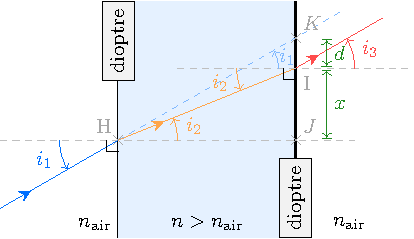
\includegraphics{vitre}
					\end{center}
				\end{tcb}
				\begin{tcb}[add to natural height=\myspace](tool){Outils}
					Loi de \textsc{Snell-Descartes}:
					\[n_1\sin i_1 = n_2\sin i_2\]
				\end{tcb}
			\end{tcbraster}
		\end{tcolorbox}
		\begin{tcolorbox}[blankest, raster multicolumn=6, space to=\myspace]
			\begin{tcbraster}[raster columns=1]
				\begin{tcb}[raster multicolumn=6](ques)'r'{Résultat attendu}
					Le rayon passe deux dioptres de l'air au verre, puis du verre à l'air.
					On utilise \textsc{Snell-Descartes} pour déterminer la direction du
					rayon émergent et la comparer à celle du rayon incident.
				\end{tcb}
				\begin{tcb}[sidebyside, righthand width=1.5cm,
						add to natural height=\myspace](appl)'r'{Application}
					\begin{itemize}[leftmargin=40pt]
						\item[\textbf{En H}] : $\sin i_1 = n\sin i_2$\smallbreak
							\hspace{-40pt}$\Leftrightarrow
								i_2 = \arcsin(\sin(i_1)/n) = \ang{28;;}$;
						\item[\textbf{Dedans}] : $i_2$ aux deux dioptres ;
						\item[\textbf{En I}] : $\sin i_3 = n\sin i_2$ ;
						\item[\textbf{D'où}] :
							$\cancel{n_1}\sin i_3 = \cancel{n_1}\sin i_1$
					\end{itemize}
					\tcblower
					Ainsi,
					\[\boxed{i_3 = i_1}\]
					(retour inverse)
				\end{tcb}
			\end{tcbraster}
		\end{tcolorbox}
	\end{tcbraster}
	\begin{enumerate}[start=3]
		\item Comme les dioptres sont parallèles, leurs normales le sont aussi.
		      Ainsi, les rayons émergent et incident sont parallèles.
		\item $\DS\tan(i_2) = \frac{\rm IJ}{\rm HJ} = \frac{x}{a}$ et $\DS\tan(i_1) =
			      \frac{x+d}{a}$, d'où $\DS\frac{d}{a} = \tan(i_1) - \frac{x}{a} =
			      \tan(i_1) - \tan(i_2)$, soit
		      \[
			      \boxed{d = a(\tan(i_1) - \tan(i_2))}
			      \quad\text{avec}\quad
			      \left\{
			      \begin{array}{rcl}
				      a   & = & \SI{5.0}{mm} \\
				      i_1 & = & \ang{45;;}   \\
				      i_2 & = & \ang{28;;}
			      \end{array}
			      \right.\]
		      C'est-à-dire
		      \[
			      \boxed{d = \SI{2.3}{mm}}
		      \]
	\end{enumerate}
}

\section{Fibre optique à saut d'indice}

\switch{
	Les câbles à fibres optiques permettent la transmission à haut débit de tous
	types de signaux électromagnétiques, sur de longues distances avec très peu
	d'atténuation~; ceux-ci se quesagent comme la lumière. Chaque câble comporte un
	grand nombre de fibres très fines.

	Une fibre optique à saut d'indice peut être assimilée à un cylindre de
	révolution d'axe $Oz$, constitué d'un cœur de rayon $a$ (de l'ordre de 8 à
	\SI{50}{\micro m}) et d'indice $n_1$, entouré d'une couche cylindrinque appelée
	\textit{gaine}, d'épaisseur $b-a$ et d'indice $n_2 < n_1$.

	\begin{figure}[h]
		\centering
		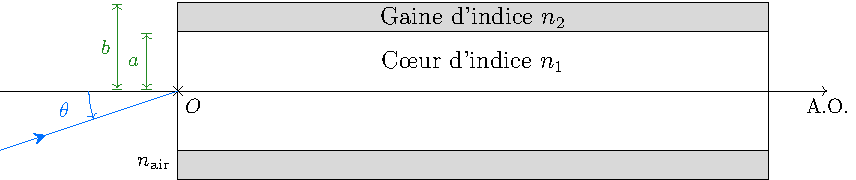
\includegraphics[width=.8\linewidth]{fibre_plain.pdf}
		\captionsetup{justification=centering}
		\caption{Schéma d'une fibre optique à saut d'indice.}
		\label{fig:fibre_plain}
	\end{figure}

	Un rayon pénètre depuis l'air dans la fibre par sa base en $O$, en faisant un
	angle $\theta$ avec l'axe optique confondu avec $Oz$.
	\begin{enumerate}
		\item Exprimer une condition sur $\theta$ en fonction des indices $n_1$ et
		      $n_2$ pour que le rayon ne se propage uniquement dans le cœur de la fibre.
		\item Déterminer l'écart temporel entre la sortie du rayon le plus rapide
		      (en ligne droite) et le rayon le plus lent ($\tt = \tt_{\lim}$).
		\item La fibre permet de transporter de très courtes impulsions lumineuses,
		      qu'on doit pouvoir distinguer à la sortie. Déterminer le débit maximal
		      d'information possible avec cette fibre en \si{Mb/s}, avec \SI{1}{b}
		      correspondant à une impulsion, avec $L = \SI{100}{km}$, $n_1 =
			      \num{1.500}$ et $n_2 = \num{1.498}$.
	\end{enumerate}
}{
	\begin{figure}[h]
		\centering
		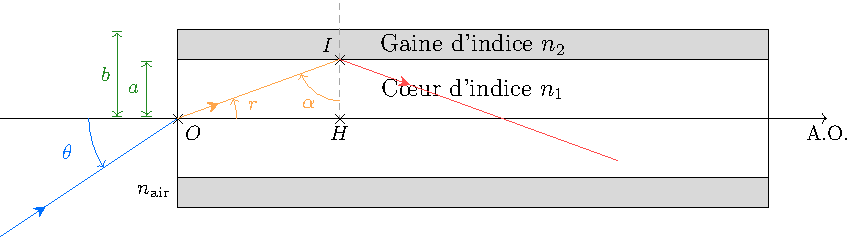
\includegraphics[width=.8\linewidth]{fibre.pdf}
		\captionsetup{justification=centering}
		\caption{Schéma d'une fibre optique à saut d'indice.}
		\label{fig:fibre}
	\end{figure}
	\begin{enumerate}
		\item
		      \begin{tcolorbox}[blankest]
			      \begin{isd}
				      \begin{itemize}

					      \item[En O] : $\sin(\theta) = n_1\sin(r) \Leftrightarrow \fbox{$\DS\sin(r) =
									      \frac{\sin(\theta)}{n_1}$}$~;
					      \item[OIH] : $\alpha = \DS \frac{\pi}{2} - r$~;
					      \item[En I] : On veut $\sin(\alpha) \geq \DS\frac{n_2}{n_1}$~;
					      \item[$\alpha\rightarrow r$] : $\sin(\alpha) = \sin(\pi/2 -r) =
							      \cos(r)$\\
						      \fbox{$\DS\sin(\alpha) \geq \frac{n_2}{n_1} \Leftrightarrow \cos(r) \geq
								      \frac{n_2}{n_1}$}
				      \end{itemize}
				      \tcblower
				      \begin{itemize}[leftmargin=100pt]
					      \item[$\cos(r)\rightarrow\sin(r)$] : $\cos^2(r) = 1-\sin^2(r)$~;
					      \item[$r\rightarrow\theta$] : $\sin^2(r) = \DS
							      \frac{\sin^2(\theta)}{n_1{}^2}$~;
					      \item[Combinaison] : $n_1{}^2 - \sin^2(\theta) \geq n_2{}^2$~;
					      \item[Conclusion] : \fbox{$\theta \leq \arcsin \left( \sqrt{n_1{}^2 -
									      n_2{}^2} \right)$}
				      \end{itemize}
				      C'est ce qu'on appelle le \textbf{cône d'acceptance}.
			      \end{isd}
		      \end{tcolorbox}
		\item Soit $L$ la longueur de la fibre optique. Un rayon entre dans la fibre
		      avec un angle d'incidence $\tt$ variable, compris entre 0 et $\tt_{\lim}$.
		      \smallbreak
		      Le rayon le plus rapide parcourt la distance $L$ à la vitesse $c/n_1$,
		      soit
		      \[
			      \boxed{T_1 = \frac{n_1L}{c}}
		      \]
		      Le rayon le plus lent arrive avec l'incidence $\tt_{\lim}$. Il parcourt
		      l'hypothénuse du triangle, soit $L/\sin(\alpha_{\lim})$, au lieu de parcourir
		      $L$. Ainsi,
		      \[
			      T_2 = \frac{n_1L}{c \sin(\alpha_{\lim})}
		      \]
		      Or, d'après la question 1, $\sin(\alpha_{\lim}) = \frac{n_2}{n_1}$. Ainsi,
		      \[
			      \boxed{T_2 = \frac{n_1{}^{2}L}{cn_2}}
		      \]
		      L'écart de temps à la réception est $\Delta{T} = T_1-T_2$, soit
		      \[
			      \boxed{\Delta{T} = \frac{n_1L}{c}\left( 1 - \frac{n_1}{n_2} \right)}
		      \]
		      C'est ce qu'on appelle la \textbf{dispersion intermodale}.
		\item Les impulsions en entrée vont être étalées de la durée $\Delta{T}$. En
		      les supposant très courtes, il faudra quand même $\Delta{T}$ pour pouvoir
		      les séparer, donc le débit sera inférieur à $1/\Delta{T}$. Pour $L =
			      \SI{100}{km}$, $n_1 = \num{1.500}$ et $n_2 = \num{1.498}$, on obtient
		      $\Delta{T} \approx \SI{1}{\micro s}$, soit un débit maximal de
		      $\SI{1}{Mb/s}$, ce qui est bien inférieur à ce que proposent les
		      fournisseurs d'accès à internet. Ainsi, en pratique on n'utilise pas de
		      fibre optique à saut d'indice pour cette raison.
	\end{enumerate}
}

\section{Mirages}
\switch{
	Cet exercice est une introduction à la quesagation de la lumière dans un milieu
	non homogène. Le but est d'interpréter qualitativement les phénomènes de mirages
	(froid et chaud). Ces illusions d'optiques apparaissent lorsque l'indice de
	l'air varie assez rapidement avec l'altitude.
	\begin{enumerate}
		\item Lorsque le sol est très «~chaud~», la température de l'air est
		      d'autant plus élevée qu'il est proche du sol. Plus la température de
		      l'air est élevée, moins son indice optique est élevé. On décompose
		      l'atmosphère en N couches planes isothermes dont l'indice optique
		      augmente avec l'altitude~:
		      \[ \forall k \in \Nb^* \quad\text{et}\quad 1 \leq k \leq N,
			      \quad n_{k+1} > n_k\]
		      \begin{minipage}{0.47\linewidth}
			      \begin{center}
				      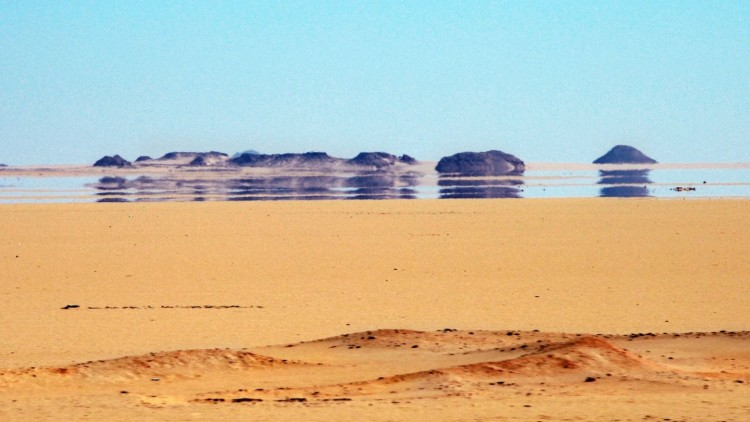
\includegraphics[width=\linewidth]{mirage_chaud}
				      \captionof{figure}{Photo d'un mirage chaud}
				      \label{fig:mir_chaud}
			      \end{center}
		      \end{minipage}
		      \hfill
		      \begin{minipage}{0.47\linewidth}
			      \begin{center}
				      \centering
				      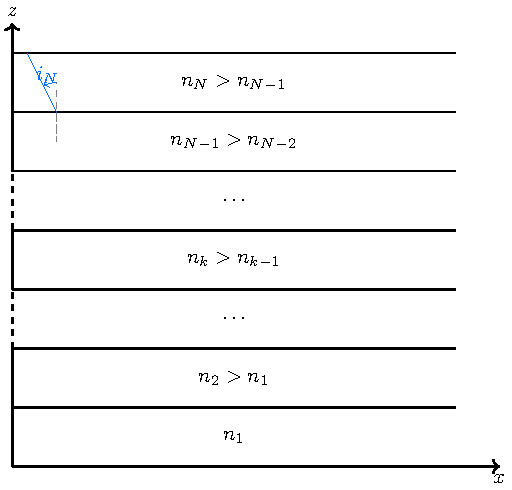
\includegraphics[height=5cm]{mirage_plain.pdf}
				      \captionof{figure}{Modèle d'atmosphère stratifié}
				      \label{fig:mirage_plain}
			      \end{center}
		      \end{minipage}
		      \begin{enumerate}
			      \item Montrer que $n_k\sin(i_k)$ est constant, où $k$ désigne la
			            $k$-ième couche atmosphérique.
			      \item Tracer les rayons réfractés par les couches d'air successives en
			            faisant apparaître les angles d'incidence et de réfraction, puis
			            montrer que pour un angle d'incidence initial suffisamment grand,
			            une réflexion totale se produit.
			      \item Pour une variation continue de l'indice $n$, tracer
			            qualitativement le trajet d'un rayon lumineux issu du ciel. Dans
			            quel sens et direction sa trajectoire est-elle courbée~?
			      \item Interpréter alors le mirage chaud observé sur la photo ci-dessus.
			            Faire un schéma.
		      \end{enumerate}

		\item Il arrive que la mer soit nettement plus «~froide~» que l'atmosphère.
		      La température de l'air augmente alors avec l'altitude. Que peut-on
		      observer si on regarde un bateau ou une île au loin~? Interpréter le
		      mirage froid de la photo page suivante. Justifier par un schéma.
		      \begin{figure}[h]
			      \centering
			      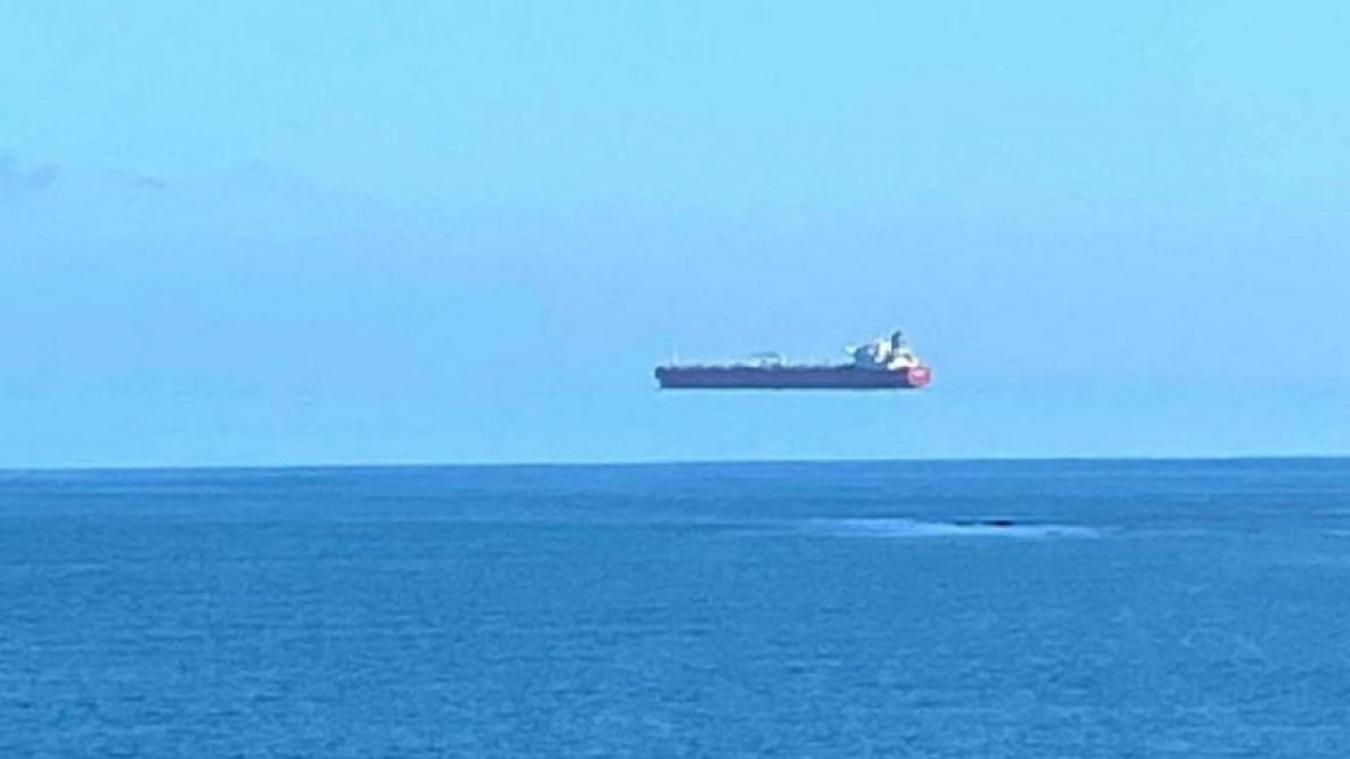
\includegraphics[width=.5\linewidth]{mirage_froid}
			      \captionsetup{justification=centering}
			      \caption{Photo d'un mirage froid}
			      \label{fig:mir_froid}
		      \end{figure}
	\end{enumerate}
}{
	\begin{wrapfigure}[13]{R}{.5\linewidth}
		\vspace*{20pt}
		\centering
		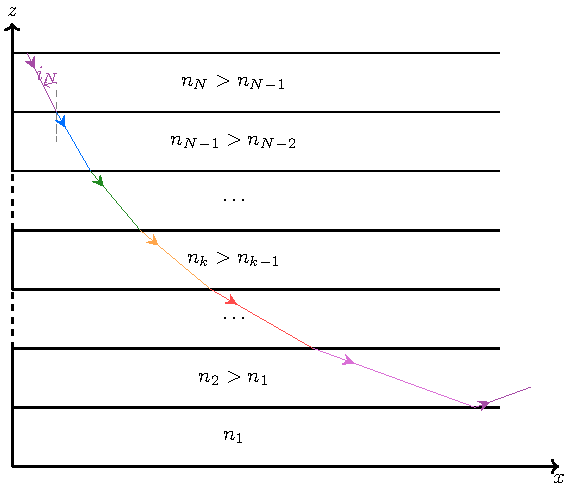
\includegraphics[width=\linewidth]{mirage}
		\captionsetup{justification=centering}
		\caption{Rayons d'un mirage chaud}
		\label{fig:mirage}
	\end{wrapfigure}
	~
	\begin{enumerate}
		\item
		      \begin{enumerate}
			      \item À chaque interface, $n_k\sin(i_k) = n_{k-1}\sin(i_{k-1})$~;
			            notamment, avec $k=2$, on a $n_2\sin(i_2) = n_1\sin(i_1)$. Ainsi,
			            tous les $n_k\sin(i_k)$ sont égaux.
			      \item Voir figure ci-après.\smallbreak
			            À chaque «~dioptre~», on a $\sin(i_{\rm lim, k}) =
				            \frac{n_{k-1}}{n_k}$. Sa valeur maximale est à $k=2$~:
			            $\sin(i_{\rm lim,2}) = \frac{n_1}{n_2}$. Comme $n_k\sin(i_k)$
			            est constant et que $n_k$ diminue, on sait que $i_k$
			            augmente~: ainsi, si l'angle d'incidence $i_N$ est
			            suffisamment grand, il y aura un $i_k$ supérieur à $i_{\rm
						            lim,2}$ et donc réflexion totale.
			      \item Voir figure.
			      \item Alors qu'on devrait voir le sable, les rayons venant du haut des
			            collines sont déviés vers le haut~: on a l'impression de voir à
			            travers la dune.
		      \end{enumerate}
	\end{enumerate}

	\begin{enumerate}[start=2]
		\item Cette fois ce sont les rayons dirigés vers le haut d'un objet lointain
		      qui sont déviés vers le bas~: on a l'impression de voir des objets
		      au-dessus du niveau de la mer. Schéma non fourni.
	\end{enumerate}
}

\section{Réfractomètre de \textsc{Pulrich}}
\switch{
	\noindent
	\begin{minipage}[t]{.68\linewidth}
		Un réfractomètre de \textsc{Pulrich} est constitué d'un bloc de verre de section
		rectangulaire d'indice $N$ connu, sur lequel on a déposé une goutte de liquide
		d'indice $n$ inconnu ($n < N$). On observe un faisceau de rayons parallèles à la
		limite réfraction/réflexion totale et on mesure en sortie l'angle $\alpha$ dans
		ce cas.
		\begin{enumerate}
			\item Établir l'expression de $n$ en fonction de $N$ et $\alpha$.
			\item Application numérique~: calculer $n$ sachant que $N = \num{1.626}$ et
			      $\alpha = \ang{60;00;}$.
		\end{enumerate}
	\end{minipage}
	\hfill
	\begin{minipage}[t]{.3\linewidth}
		~
		\vspace*{-20pt}
		\begin{center}
			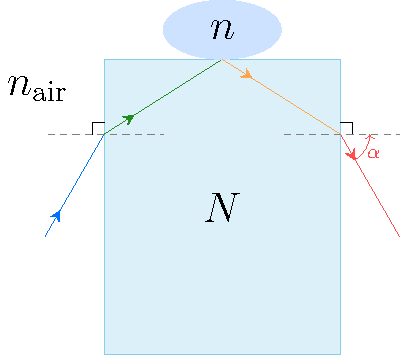
\includegraphics[width=\linewidth]{pulrich_plain}
			\label{fig:pulrich_plain}
		\end{center}
	\end{minipage}
}{
	\noindent
	\begin{minipage}[t]{.68\linewidth}
		\begin{enumerate}
			\item $\DS \sin(i_{\rm lim, N\rightarrow n}) = \frac{n}{N}$ d'une part.
			      D'autre part, $N\sin(\theta) = \sin\alpha$, mais on a aussi $\theta =
				      \pi/2 - i_{\rm lim}$~: on a donc $\sin\theta = \cos i_{\rm lim} = \DS
				      \sqrt{1- \left(\frac{n}{N}\right)^2}$. Ainsi, $\DS\sin^2\alpha = N^2
				      \left( 1 - \frac{n^2}{N^2} \right)$~; autrement dit,
			      \begin{equation*}
				      \boxed{n = \sqrt{N^2 - \sin^2\alpha}}
				      \quad\text{avec}\quad
				      \left\{
				      \begin{array}{rcl}
					      N      & = & \num{1.622} \\
					      \alpha & = & \ang{60;;}
				      \end{array}
				      \right.
			      \end{equation*}
			\item Application numérique~:
			      \[\boxed{n = \num{1.376}}\]
		\end{enumerate}
	\end{minipage}
	\hfill
	\begin{minipage}[t]{.3\linewidth}
		~
		\begin{center}
			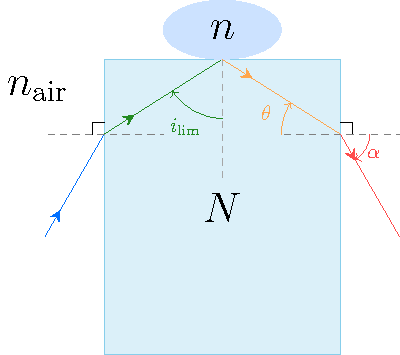
\includegraphics[width=\linewidth]{pulrich}
			\label{fig:pulrich_plain}
		\end{center}
	\end{minipage}
}

\section{Incidence de Brewster}
\switch{
	Un dioptre plan séparer l'air d'un milieu d'indice $n$. Pour quelle valeur de
	l'angle d'incidence le rayon réfléchi est-il perpendiculaire au rayon réfracté~?
}{
	Les rayons réfléchis et réfractés sont perpendiculaires si $r+i =
		\frac{\pi}{2} \Leftrightarrow r = \frac{\pi}{2} -i$. En venant de l'air, on a
	$\sin i = n\sin r$, soit $\sin i = n\cos i$~; autrement dit
	\begin{equation*}
		\boxed{\tan i = n}
	\end{equation*}
}

\section{Réfraction et dispersion}
\switch{
	Un rayon lumineux, se propageant dans l'air, arrive avec une incidence $i =
		\ang{40;;}$
	sur un dioptre air/verre plan. Si on considère que ce rayon est constitué de
	lumière blanche, calculer l'écart angulaire entre les rayons réfractés extrêmes.

	\textit{Données}~: l'indice du verre est donné par la formule de Cauchy~: $\DS n
		= A + \frac{B}{\lambda_0{}^2}$, avec $A = \num{1.504}$ et $B =
		\SI{4.188e-15}{m^2}$~; l'indice de l'air est $n_{\rm air} = \num{1.000}$.
}{
	La lumière blanche est constituée d'une superposition de longueurs d'onde dans
	le vide entre \SIrange{400}{800}{nm}. Quand ce faisceau arrive sur le dioptre et
	passe dans le milieu, l'indice de réfraction, qu'on utilise dans la relation de
	\textsc{Snell-Descartes}, change selon la longueur d'onde dans le vide. Pour une
	même valeur de $i$ incident on aura donc deux valeurs extrêmes de $r$ réfracté,
	que l'on nomme $r_b$ et $r_r$ pour «~bleu~» et «~rouge~», selon~:

	\begin{minipage}{0.49\linewidth}
		\begin{empheq}[box=\fbox]{align*}
			n_{\rm air}\sin(i) &= n_b\sin(r_b)\\
			n_{\rm air}\sin(i) &= n_r\sin(r_r)
		\end{empheq}
	\end{minipage}
	$\Longleftrightarrow$
	\begin{minipage}{0.49\linewidth}
		\begin{empheq}[box=\fbox]{align*}
			r_b &= \arcsin \left( \frac{n_{\rm air}\sin(i)}{n_b} \right)\\
			r_r &= \arcsin \left( \frac{n_{\rm air}\sin(i)}{n_r} \right)
		\end{empheq}
	\end{minipage}

	Comme $\lambda_{0,b} < \lambda_{0,r}$, $\underbrace{n(\lambda_{0,b})}_{n_b} >
		\underbrace{n(\lambda_{0,r})}_{n_r}$ et
	forcément $r_b < r_r$. On calcule~:

	\begin{minipage}{0.49\linewidth}
		\begin{empheq}[box=\fbox]{align*}
			n_b &= \num{1.53}\\
			n_r &= \num{1.51}
		\end{empheq}
	\end{minipage}
	$\Longleftrightarrow$
	\begin{minipage}{0.49\linewidth}
		\begin{empheq}[box=\fbox]{align*}
			r_b &= \ang{24.8;;}\\
			r_r &= \ang{25.2;;}
		\end{empheq}
	\end{minipage}

	L'écart angulaire est donc
	\[\boxed{\theta = r_r - r_b = \ang{0.35;;}}\]

	\begin{figure}[h]
		\centering
		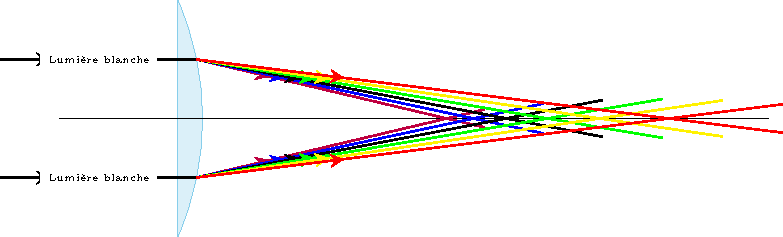
\includegraphics[width=.61\linewidth]{abbe_chroma.pdf}
		\captionsetup{justification=centering}
		\caption{Exemple (exagéré) de dispersion (aberration chromatique).}
		\label{fig:aberr}
	\end{figure}
}


\end{document}
